\section{Study Results}
\subsection{Objectives}
In order to assess the feasbility of extending the KCFN to the Swope Corridor,
it is essential to define well-established targets for any potential work. The
proposal that follows is intended to satisfy the following parameters:
\begin{description}
\item[Purpose] This proposal is for a project intended to improve the state of
connectvity for businesses and residents within the Swope Corridor, establish
the Mary Kelley Center as a local hub for connectivity and digital skills
education, and demonstrate an organizing model that can be replicated in other
 communities.
\item[Scope] The geographical area under consideration is bounded by Volker
Boulevard and Swope Parkway on the North, Swope Parkway/Cleveland Street
on the East, 63\textsuperscript{rd} Street on the South, and The Paseo on the West
-- a total area of 7km\textsuperscript{2}. In addition to The Upper Room, it 
should involve an array of area residents, businesses, non-profits, and community groups.
\item[Coverage] Outside of bringing a cost-effective ultra-broadband connection
to the Kelly Center, the paramount concern is improving the availability of 
affordable residential Internet service for those within the designated geographic
scope. While it isn't possible to guarantee coverage to \%100 of residences with a community network approach,
our objective should be to allow any and all blocks within the area to participate. This
will not be possible without significant investment and involvement from within the
community itself.
\item[Functionality] Those that elect to participate in the network, in addition
to gaining access to resouces published on the KCFN, should have the
ability to purchase low-cost Internet access. 
\item[Performance] While exact performance figures will depend case-by-case on a
number of factors, the KCFN should enable broadband connectivity capable of supporting
telephony, web 2.0, and multimedia applications.
\item[Cost] The total cost of
accessing the Internet via the KCFN, including hardware, should be lower than existing
alternatives over the course of one year.
\item[Sustainibility] Above all, this effort should aim to foster a digital commons
that is sustainable in the long term --- focusing first and foremost on education, grassroots
support, and the capacity for ongoing, organic growth.
\end{description}
\subsection{Survey Information}
The primary physical considerations in determining build feasibility and an
appropriate course of action are topographic terrain and RF environment. We
surveyed the target area in October and November of 2013, analyzing the lay of the land
and assesing spectrum availability. \par
\subsubsection{Terrain}
The terrain in question presents certain significant challenges to network
deployment. The Kelly Center's vista over the Town Fork Creek neighborhood
will significantly aid in deployment there, covering a great many points
south and east. The challenge will be in Blue Hills neighborhood, especially 
west of Wabash Avenue. While the terrain does not preclude network deployment
it will necessitate an effort to establish relays in the vicinity of 49\textsuperscript{th}
\& Euclid and 57\textsuperscript{th} \& Woodland.
\begin{center}
\fbox{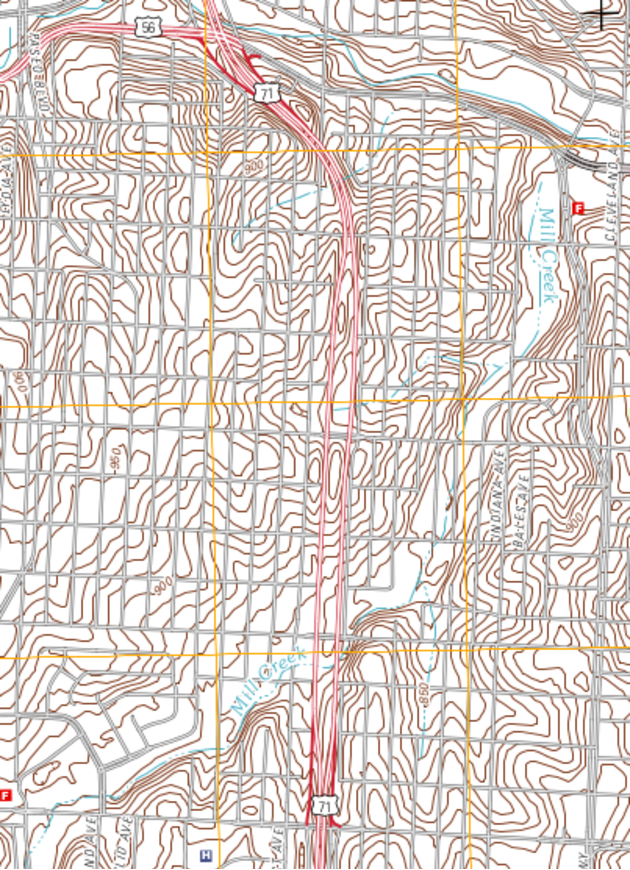
\includegraphics[width=4in]{./images/UR_topo.pdf}}
\end{center}
\begin{center}
\fbox{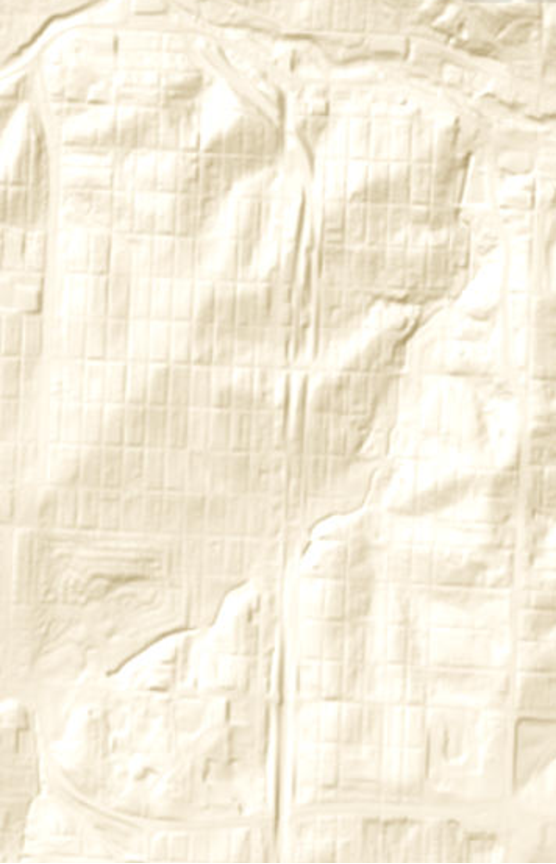
\includegraphics[width=4in]{./images/UR_hill_shade.pdf}}
\end{center}
\subsubsection{RF Environment}
The RF enviornment shows light to moderate utilization in the 5GHz band. Our
finding is that while appropriate channel selection and efficiency will be critical,
there is ample spectrum available for use in the target geography. In order to
assess spectrum health, we conducted sector surveys from the roof of the Kelly Center. \par
The graph below reflects the noise and signal levels in the 5GHz spectrum in the direction
of St. Mary's Church, at 31\textsuperscript{st} \& Troost. All but 20MHz worth of spectrum
is deemed usable, with a noise floor well below 90dBm:
\begin{center}
\fbox{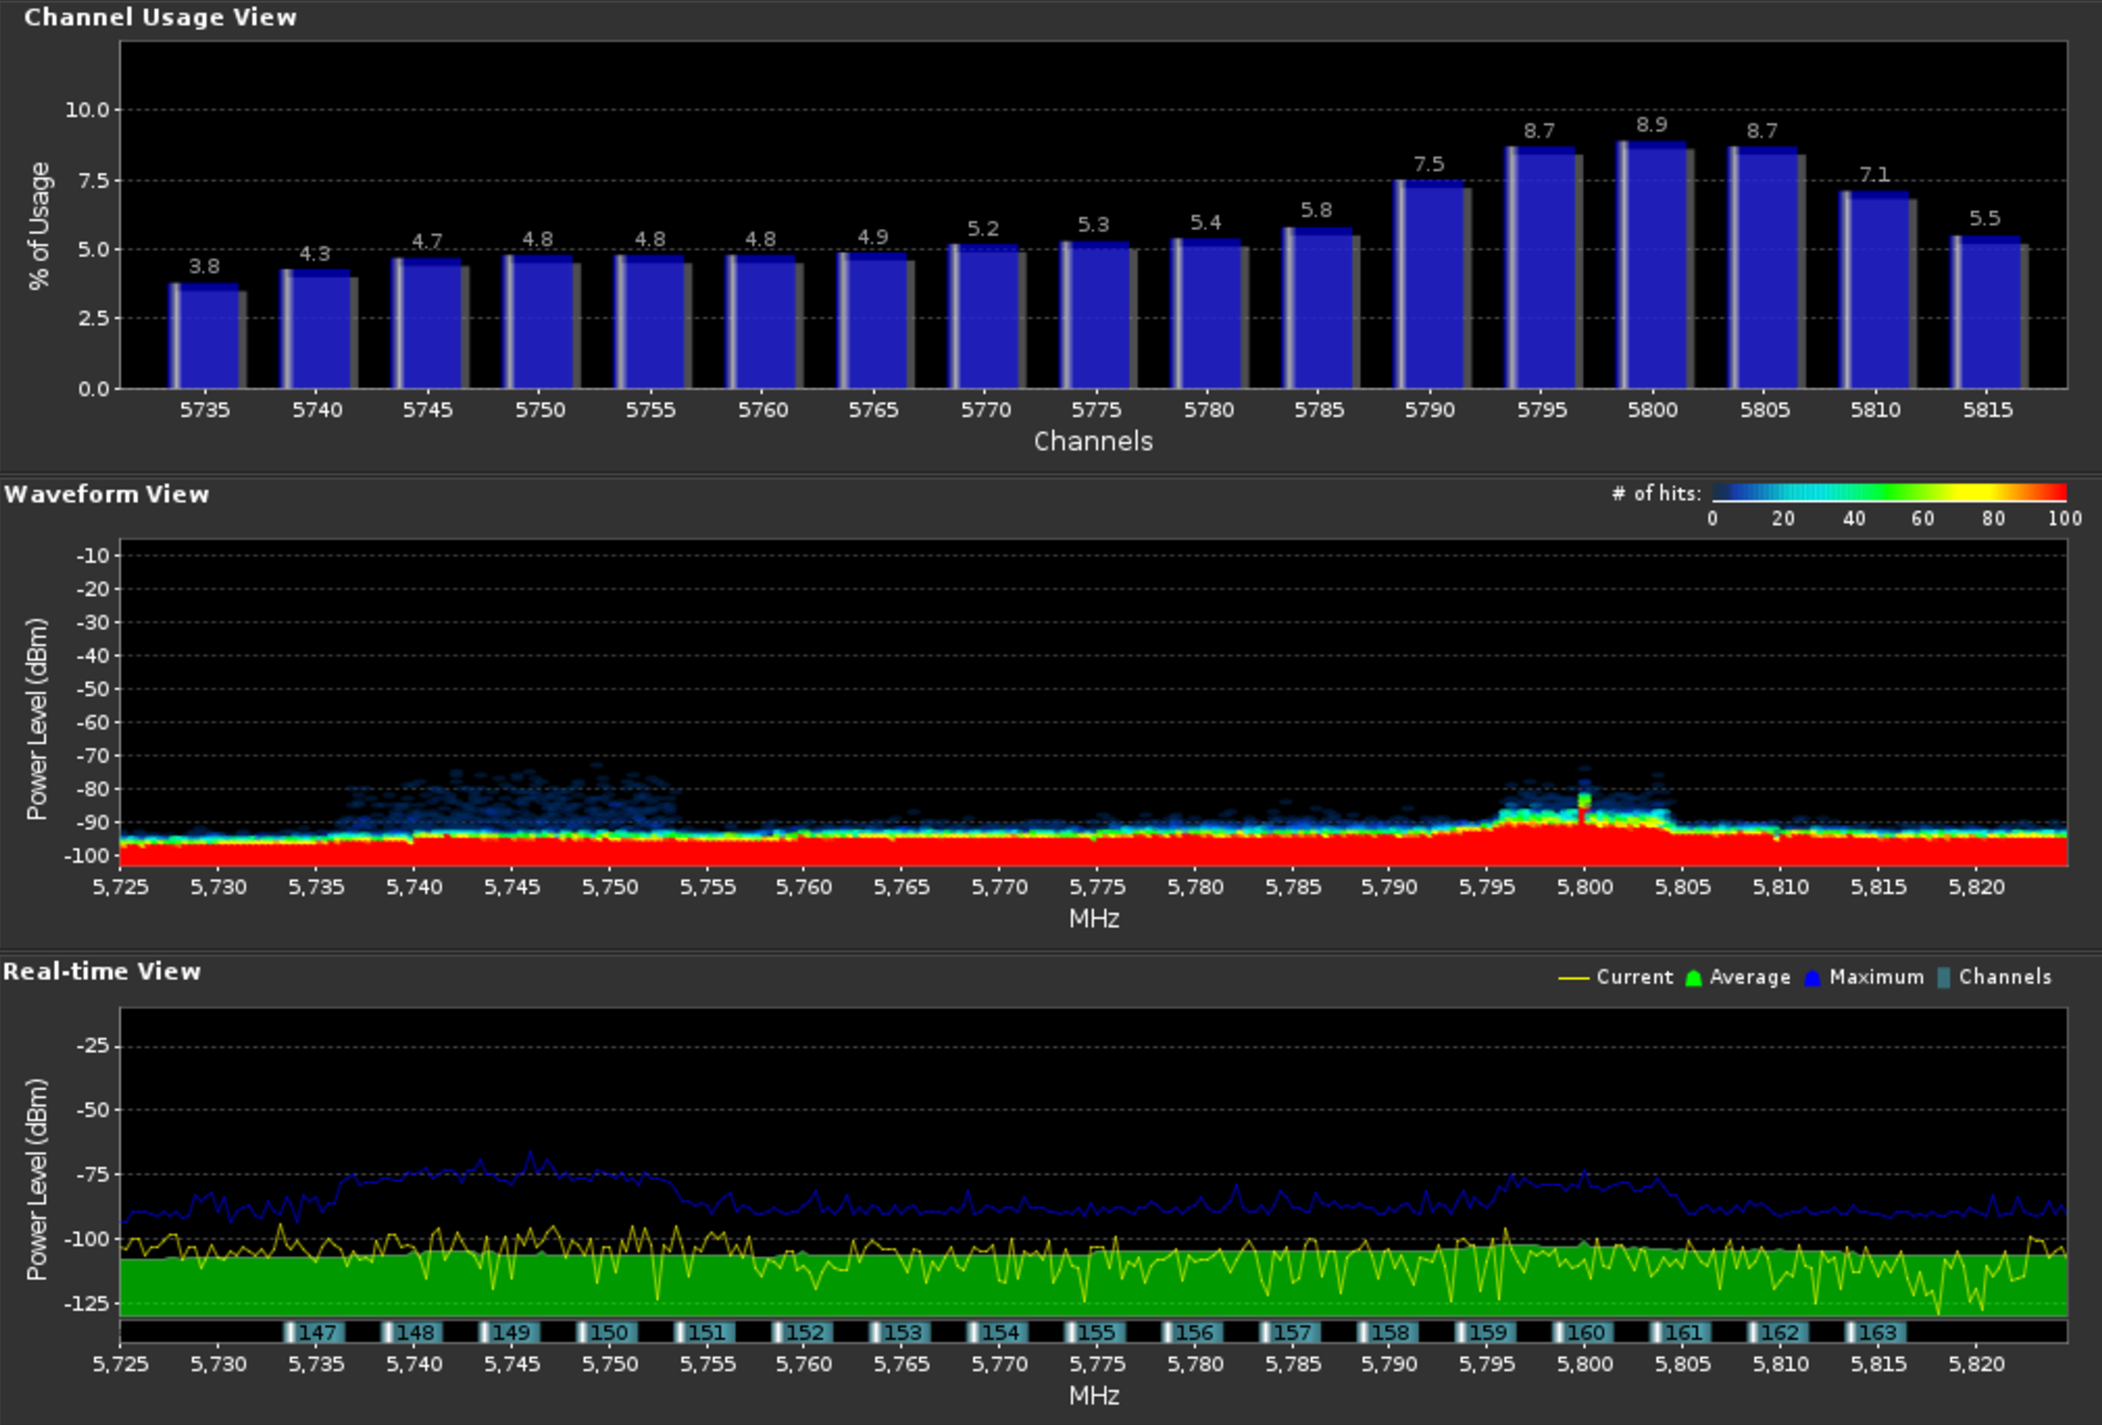
\includegraphics[width=5in]{./images/to3101_rf_airview_crop.pdf}}
\end{center}
The next graph shows the situation in the direction of the DuBois Learning Center, at 
55\textsuperscript{th} \& Cleveland. The spectrum from 5.775GHz to 5.8GHz is not usable, but the rest of the band remains usable:
\begin{center}
\fbox{\includegraphics[width=5in]{./images/to_dubois_airview_crop.pdf}}
\end{center}
Next, in the direction of Southeast High, we see the same sitation as above, with the band from 5.775GHz to 5.8GHz saturated, but the rest of the available frequencies in good shape:
\begin{center}
\fbox{\includegraphics[width=5in]{./images/to_southeasthigh_airview_crop.pdf}}
\end{center}
Finally, looking due west, towards Blue Hills, we see that the entire spectrum is usable, though it does have a slightly higher noise floor, generally approaching 90dBm:
\begin{center}
\fbox{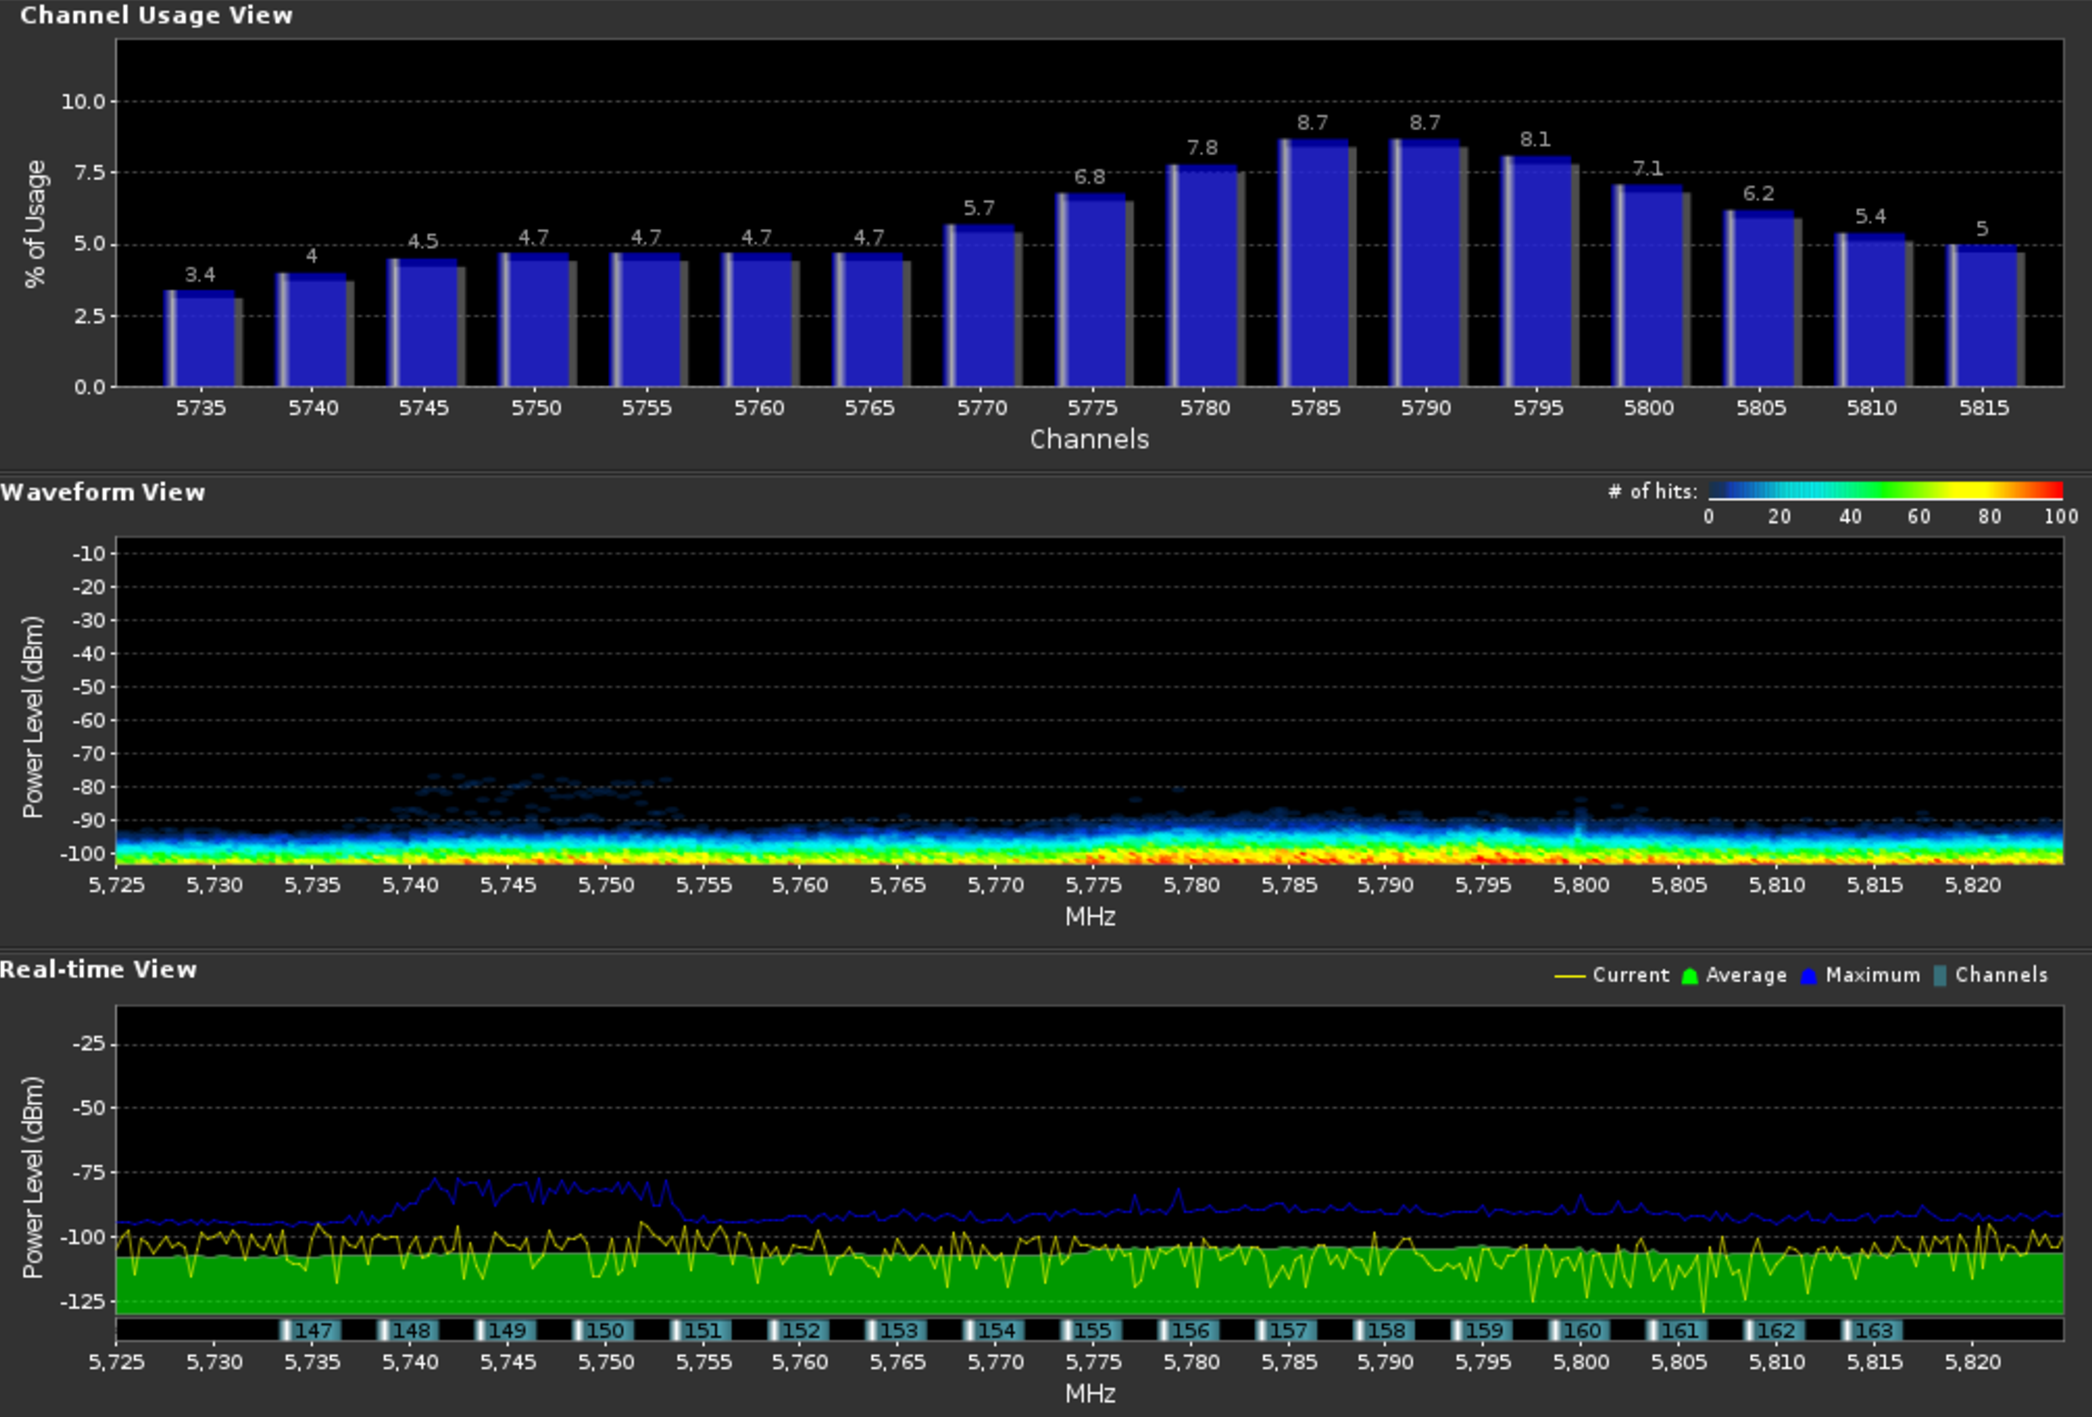
\includegraphics[width=5in]{./images/due_west_airview_crop.pdf}}
\end{center}
We did not survey the 24GHz spectrum that we plan to use for backhaul, because it will be precisely aligned, and should not suffer from interference, as it is not widely deployed.
\subsection{Findings}
On the basis of our survey results and prior field experience, we have devised
a proposed plan of action and associated cost estimates. These projections are intended
to serve as a starting point for collaboration, and certainly do not reflect the
only viable path towards accomplishing the stated objectives.\par
\subsubsection{Proposed Plan}
\begin{description}
\item[Phase I - Spring 2014]
\item[Phase II - Summer/Fall 2014]
\item[Phase III - 2015 \& Beyond]
\subsubsection{Costs and Figures}
